
\subsection{Double Blast Test}

The double blast test was introduced by Woodward \& Colella in 1984. It is a one-dimensional test of two strongly
interacting shock fronts. Except for very early times, it does not have an analytic solution \& convergence is
usually measured by comparison to a very highly refined grid.

\subsubsection{Initial conditions}

The domain consists of a grid $x \in [0, 1]$. The initial conditions for the test are:
\begin{itemize}
\item $\rho(x) = 1$
\item $\vec{v}(x) = \vec{0}$
\item $P(x < 0.1) = 100$
\item $P(0.1 \le x \le 0.9) = .01$
\item $P(x > 0.9) = 1000$
\item Gamma-law gas, $\gamma = 7/5$
\end{itemize}

Two extremely strong shocks are launched towards the center. Repeated collisions between shocks and contact
discontinuities generate an extremely complex flow with very fine details which is extremely difficult to reproduce
on an Eulerian grid without immense levels of refinement.

\subsubsection{Analysis}

\begin{figure*}
\begin{center}
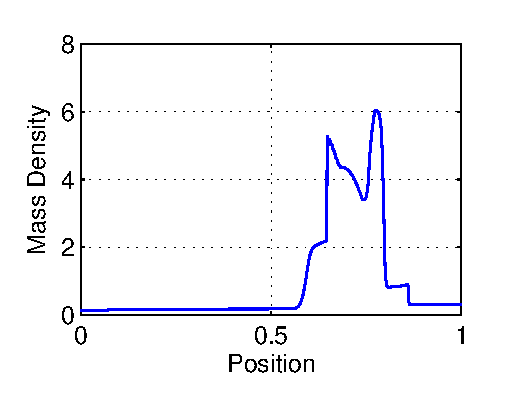
\includegraphics{DoubleBlast.eps}
\caption{Double Blast at t = 0.038}
\end{center}
\end{figure*}
\subsubsection{Initial Conditions}

Boundary conditions on both ends of the domain are mirror.

Imogen's runfile parameters are
\begin{itemize}
\item \tt{pLeft} - Sets the initial pressure in the left tenth of the grid
\item \tt{pMid} - Sets the ambient pressure
\item \tt{pRight} - Similarly sets the pressure in the right tenth of the grid
\end{itemize}

The default values are those of Woodward/Colella, \begin{tt}pLeft = 100\end{tt}, \begin{tt}pMid = .01\end{tt}
and \begin{tt}pRight = 1000\end{tt}.

Further reading:
Woodward/Colella 1984
